\section{Introduction}
\label{sec:introduction}
Inpainting is an image processing technique used to infer the value of unknown pixels using the information apparent in the original image. One application for this method is image restoration where single pixels or larger scratches are missing, e.g. due to defective image acquisition or the age-driven deterioration of video footage. Another very common application is the removal of certain parts of an image, like watermarks or user-selected objects in the image. Figure \ref{fig:apps} shows examples for input images that can be treated by inpainting methods. Throughout this paper we assume that it is known beforehand which pixels have to be reconstructed. The extraction of defective regions in the image is not discussed here.

\begin{figure*}[t]
	\centering
	\begin{subfigure}{.5\columnwidth}
	   \centering
	   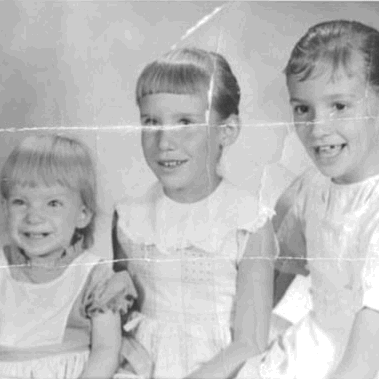
\includegraphics[width=.9\columnwidth]{graphics/3children_original_cropped.png}%
	      \caption{Image restoration
	      \label{fig:apps:image_restoration}
	   }
	\end{subfigure}\hfill%
	\begin{subfigure}{.5\columnwidth}
	   \centering
	   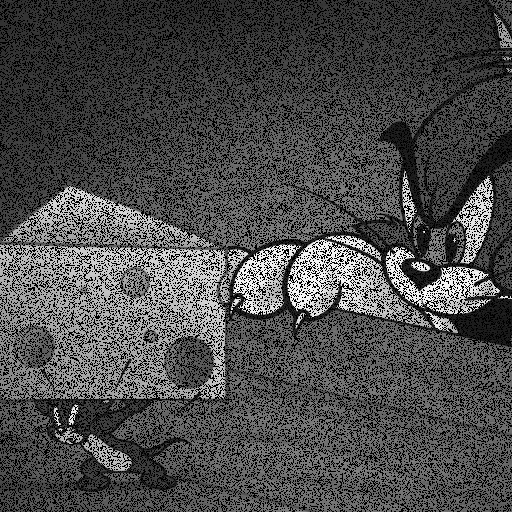
\includegraphics[width=.9\columnwidth]{graphics/TomAndJerry_512x512_pepper_in.png}%
	      \caption{Noise removal
	      \label{fig:apps:noise_removal}
	   }
	\end{subfigure}\hfill%
	\begin{subfigure}{.5\columnwidth}
	   \centering
	   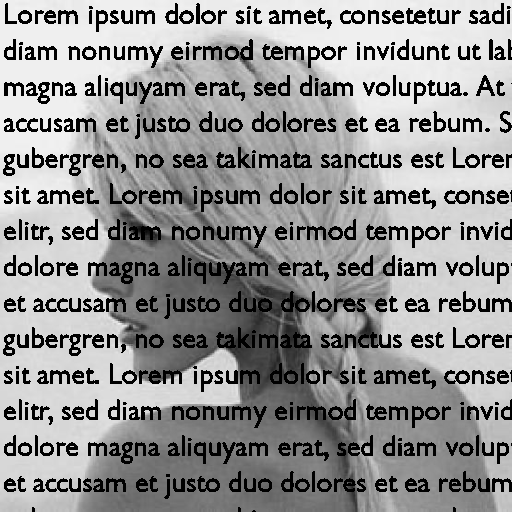
\includegraphics[width=.9\columnwidth]{graphics/claudia_512x512_mask_in.png}%
      	   \caption{Removal of watermarks
	      \label{fig:apps:watermarks}
	   }
	\end{subfigure}\hfill%
	\begin{subfigure}{.5\columnwidth}
	   \centering
	   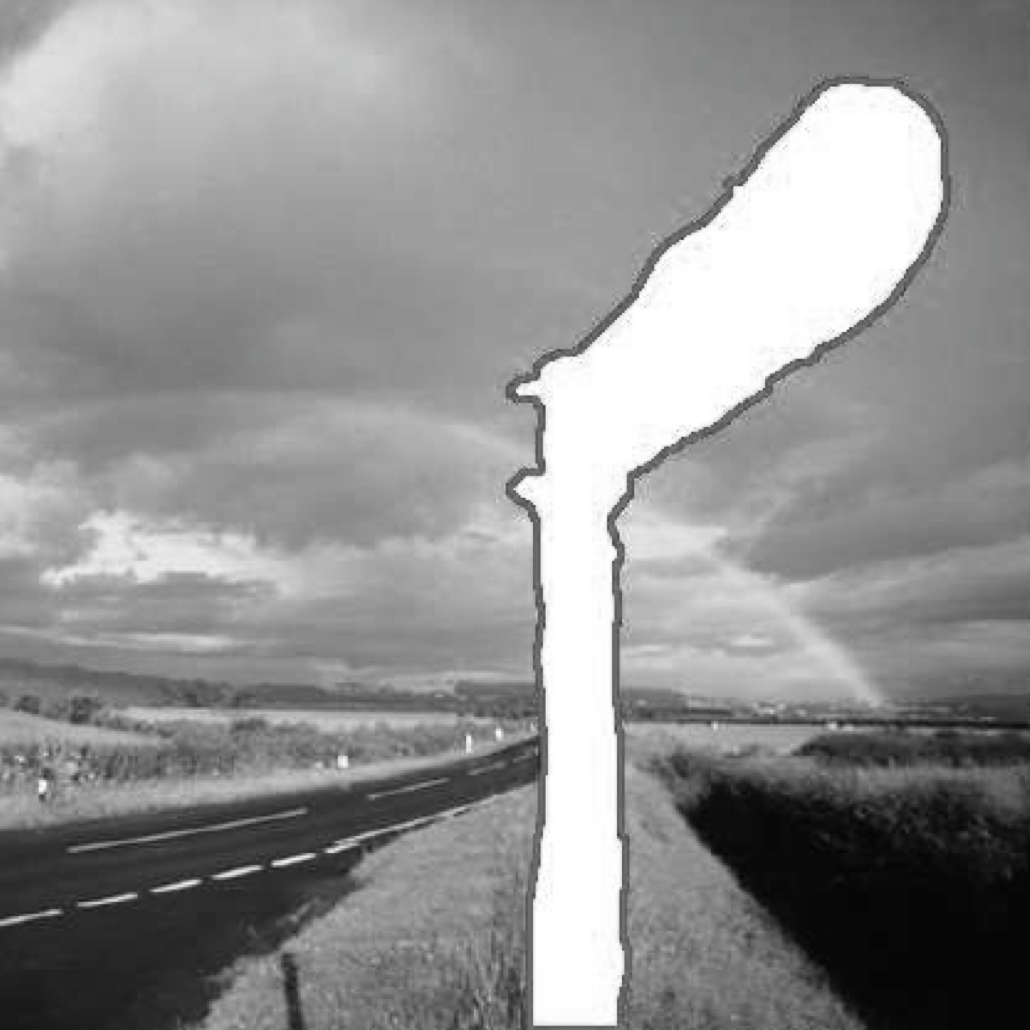
\includegraphics[width=.9\columnwidth]{graphics/object_removal_gray.png}%
      	   \caption{Object removal
	      \label{fig:apps:object_removal}
	   }
	\end{subfigure}\hfill%
	\caption{Sample applications for inpainting. (Images \ref{fig:apps:image_restoration}), \ref{fig:apps:noise_removal}), and \ref{fig:apps:watermarks}) are taken from \cite{CIL2015}, \ref{fig:apps:object_removal}) is from \cite{criminisi2004region})
	   \label{fig:apps}
	}
\end{figure*}

\mypar{Existing work}
Many different techniques exist for inpainting, see for example \cite{tauber2007review} for a review of methods originating in the domain of computer vision. A very common approach is referred to as \textit{texture-synthesis} where the objective is to remove (potentially large) objects from an image by mimicking the surrounding region of the to-be-removed objected. Very popular in the image processing community is the method described by Criminisi et al. \cite{criminisi2004region}, an onion-peel approach where local gradients steer the fill-in procedure, which helps to not only preserve texture but also structure.

Recently, inpainting driven by sparse encoding, a concept from the domain of statistical learning, became popular, see for example \cite{fadili2009inpainting} or \cite{elad2005simultaneous}. 

\mypar{Our approach}
The method presented here is based on sparse coding of image patches, which we combine with ideas that are inspired by the works of \cite{criminisi2004region}. The novelty of our patch-based method consists of the combination of the following components:
\begin{itemize}
   \item Valuable Information Propagation (VIP): Use evidence found in neighbouring patches for the sparse coding.
   \item Confidence Blending (CB): Redundant reconstruction of missing pixels by overlapping patches.
   \item A scheme to learn under-complete dictionaries that allow a reliable and fast encoding.
\end{itemize}

\mypar{Structure of the text} In section \ref{sec:methods} the proposed method is presented in depth. Section \ref{sec:results} presents our implementation which is then discussed in the subsequent section \ref{sec:discussion}. 